\documentclass[a4paper,12pt]{article}
%% Работа с русским языком
\usepackage{cmap}                   % поиск в PDF
\usepackage{mathtext}               % русские буквы в формулах
\usepackage[T2A]{fontenc}           % кодировка
\usepackage[utf8]{inputenc}         % кодировка исходного текста. НИКОГДА НЕ МЕНЯТЬ.
\usepackage[english,russian]{babel} % локализация и переносы
\usepackage{epigraph}               % делать эпичные эпиграфы
\usepackage{fancybox,fancyhdr}      % для колонтитулов
\usepackage{multicol}
\usepackage{float}
%% Отступы между абзацами и в начале абзаца 
\setlength{\parindent}{0pt}
\setlength{\parskip}{\medskipamount}

%% Изменяем размер полей
\usepackage[top=0.7in, bottom=0.75in, left=0.625in, right=0.625in]{geometry}

%% Изменяем размер отступов колонтитулов
\renewcommand{\headrulewidth}{1.8pt}
\renewcommand{\footrulewidth}{0.0pt}

%% Графика
\usepackage[pdftex]{graphicx}
\graphicspath{{images/}}

%% Различные пакеты для работы с математикой
\usepackage{mathtools}      % Тот же amsmath, только с некоторыми поправками

\usepackage{amssymb}        % Математические символы
\usepackage{amsthm}         % Пакет для написания теорем
\usepackage{amstext}
\usepackage{array}
\usepackage{amsfonts}
\usepackage{icomma}         % "Умная" запятая: $0,2$ --- число, $0, 2$ --- перечисление
\usepackage{enumitem}       % Для выравнивания itemize (\begin{itemize}[align=left])
\usepackage{wrapfig} 
% Номера формул
\mathtoolsset{showonlyrefs=true} % Показывать номера только у тех формул, на которые есть \eqref{} в тексте.

% Ссылки
\usepackage[colorlinks=true, urlcolor=blue, bookmarks=false]{hyperref}

% Шрифты
\usepackage{euscript}  % Шрифт Евклид
\usepackage{mathrsfs}  % Красивый матшрифт

% Свои команды\textbf{}
\DeclareMathOperator{\sgn}{\mathop{sgn}}

% Перенос знаков в формулах (по Львовскому)
\newcommand*{\hm}[1]{#1\nobreak\discretionary{}
{\hbox{$\mathsurround=0pt #1$}}{}}

% Графики
\usepackage{tikz}

% Изменим формат \section и \subsection:
\usepackage{titlesec}
\titleformat{\section}
{\vspace{1cm}\centering\LARGE\bfseries} % Стиль заголовка
{}                        % префикс
{0pt}                     % Расстояние между префиксом и заголовком
{}                        % Как отображается префикс
\titleformat{\subsection} % Аналогично для \subsection
{\Large\bfseries}
{}
{0pt}
{}

%% Титульный лист
\renewcommand{\maketitle}{\begingroup
    \hbox{
        \hspace*{0.12\textwidth}
        \rule{1pt}{\textheight}
        \hspace*{0.05\textwidth}
        \parbox[b]{0.775\textwidth}{
            {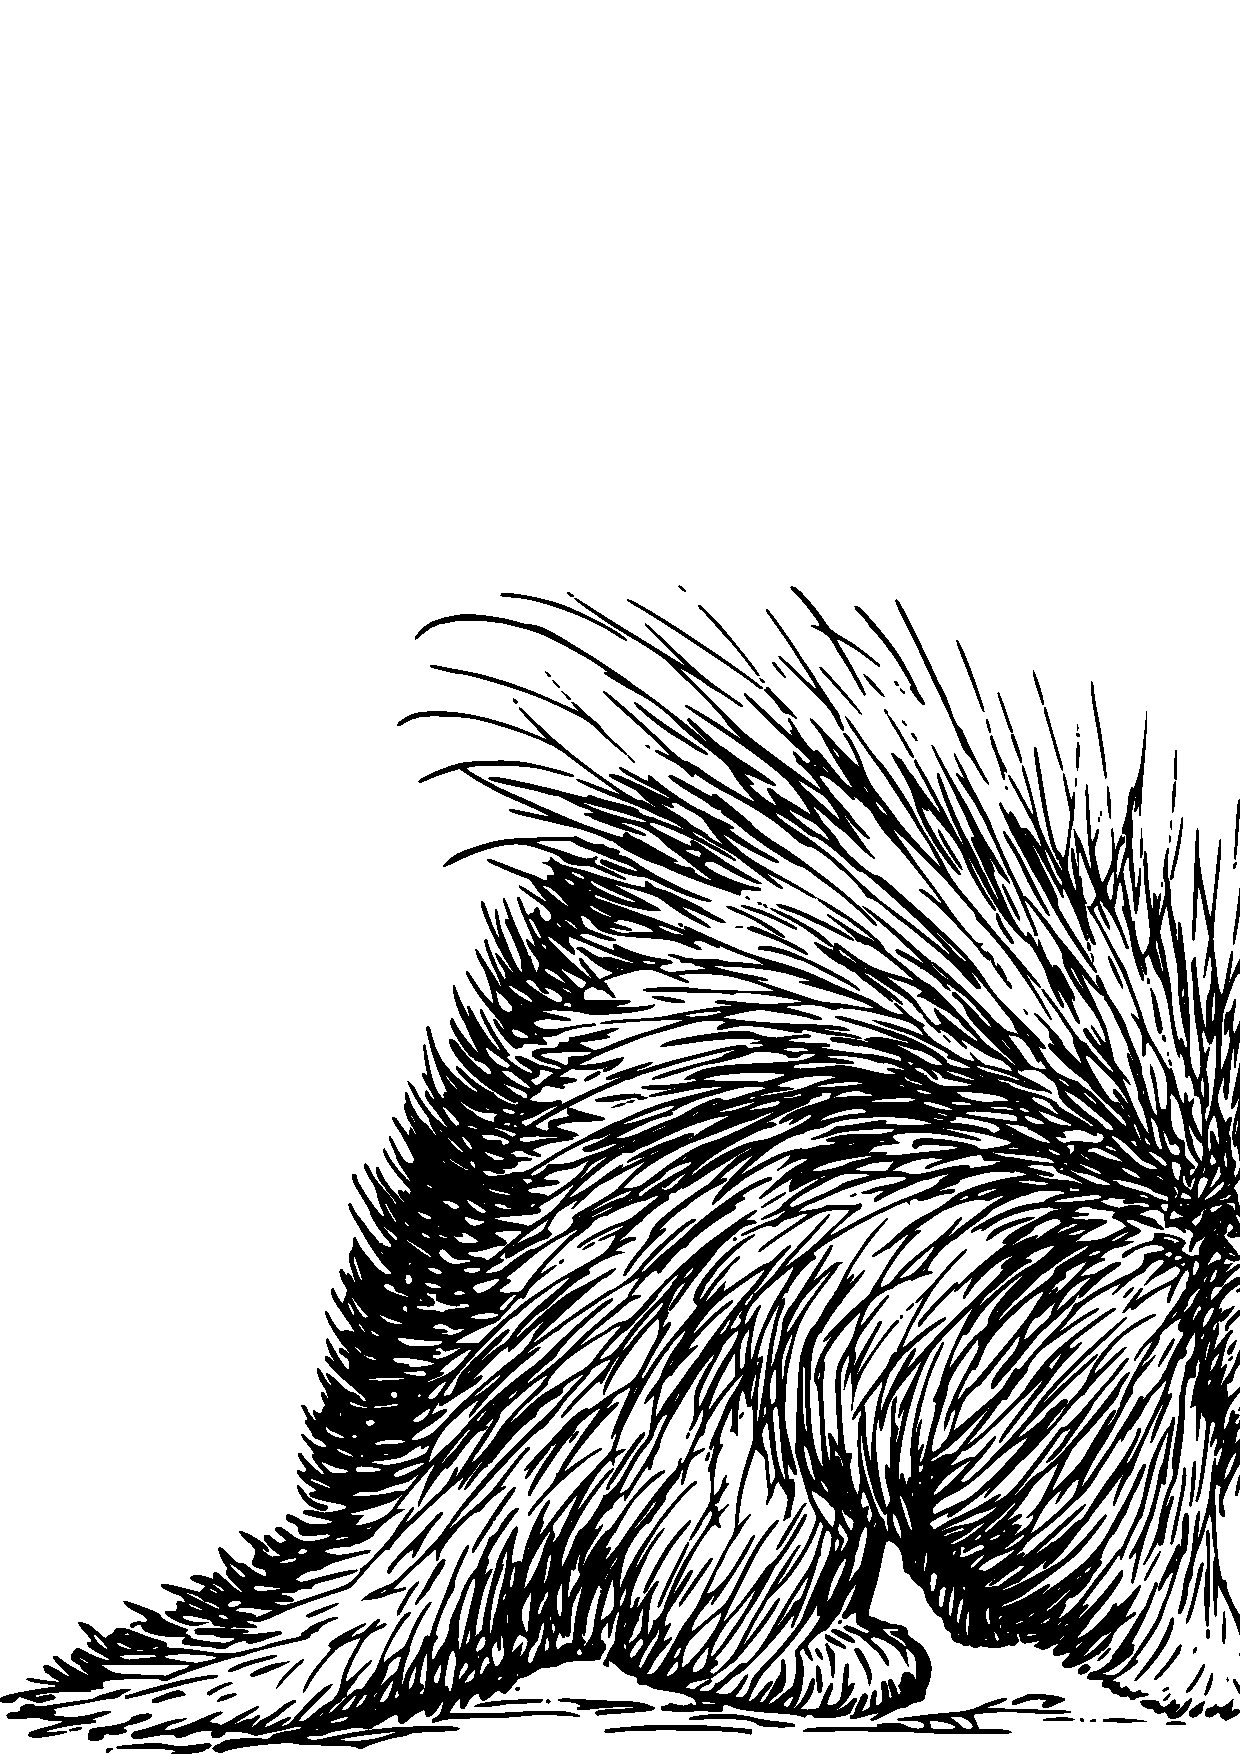
\includegraphics[width=\linewidth]{images/Title.png}}\\[2\baselineskip]
            {\noindent\Huge\bfseries Математический анализ}\\[\baselineskip]
            {\large\textrm{Конспекты лекций}}\\[3\baselineskip]
            {\Large\textsc{Лектор: В.В. Галатенко}}\\[\baselineskip]
            {Конспекты вели Дискин Михаил, Анастасия Иовлева и Руслан Хайдуров}\\[6\baselineskip]
            {\noindent НИУ ВШЭ, 2016-2017}\\[\baselineskip]
        }
    }
    \endgroup
}

\usepackage{mathdots}
\usepackage{floatflt}
\setlength{\headheight}{15pt}
%% Для колонтитула
\def\head{
{\it \small НИУ ВШЭ $\bullet$ Факультет компьютерных наук $\bullet$ Прикладная математика и информатика}}

%% Делаем верхний и нижний колонтитулы
\fancyhf{}
\fancyhead[R]{\head}
\fancyfoot[L]{{\small {\it М. Дискин, А. Иовлева, Р. Хайдуров. Математический анализ-3}}}
\fancyhead[L]{\thepage}
\fancyfoot[R]{{\small {\it Лекция \thesection }}}



%% Теоремы и иже с ними
\theoremstyle{remark}
\newtheorem*{Comment}{Примечание}
\newtheorem*{Task}{Упражнение}
\newtheorem*{Examples}{Пример}
\newtheorem*{Designation}{Обозначение}

\theoremstyle{definition}
\newtheorem{Def}{Определение}

\theoremstyle{plain}
\newtheorem{Lemma}{Лемма}
\newtheorem{Theorem}{Теорема}
\newtheorem{Test}{Признак}
\newtheorem*{Statement}{Утверждение}
\newtheorem{Problem}{Задача}
\newtheorem*{Hypothesis}{Гипотеза}
\newtheorem*{Consequence}{Следствие}
\newtheorem{Properties}{Свойство}



\newcommand{\0}{\vec{0}}
\renewcommand{\Re}{\mathrm{Re\:}}
\renewcommand{\Im}{\mathrm{Im\:}}
\newcommand{\Arg}{\mathrm{Arg\:}}
\renewcommand{\arg}{\mathrm{arg\:}}
\newcommand{\Mat}{\mathrm{Mat}}
\newcommand{\id}{\mathrm{id}}
\newcommand{\isom}{\xrightarrow{\sim}} 
\newcommand{\leftisom}{\xleftarrow{\sim}}
\newcommand{\Hom}{\mathrm{Hom}}
\newcommand{\Ker}{\mathrm{Ker}\:}
\newcommand{\rk}{\mathrm{rk}\:}
\newcommand{\diag}{\mathrm{diag}}
\newcommand{\ort}{\mathrm{ort}}
\newcommand{\pr}{\mathrm{pr}}
\newcommand{\vol}{\mathrm{vol\:}}
\def\limref#1#2{{#1}\negmedspace\mid_{#2}}
\newcommand{\eps}{\varepsilon}

\renewcommand{\phi}{\varphi} % плохо, так как есть \phi в англ раскладке.
\newcommand{\e}{\mathbb{e}}
\renewcommand{\l}{\lambda}
\newcommand{\N}{\mathbb{N}}
\newcommand{\Z}{\mathbb{Z}}
\newcommand{\Q}{\mathbb{Q}}
\newcommand{\R}{\mathbb{R}}
\renewcommand{\C}{\mathbb{C}}
\newcommand{\E}{\mathbb{E}}
\newcommand{\B}{\mathcal{B}}
\newcommand{\D}{\mathcal{D}}
\newcommand{\Ri}{\mathcal{R}}  % Риман

\newcommand{\vvector}[1]{\begin{pmatrix}{#1}_1 \\\vdots\\{#1}_n\end{pmatrix}}
\renewcommand{\vector}[1]{({#1}_1, \ldots, {#1}_n)}

\newcommand{\rarr}{\rightarrow}
\renewcommand{\leq}{\leqslant}
\renewcommand{\geq}{\geqslant}
\renewcommand{\le}{\leqslant}
\renewcommand{\ge}{\geqslant}
\renewcommand{\d}{\mathrm{d}}
\newcommand{\x}{\hat{x}}
\newcommand{\y}{\hat{y}}

\newcommand{\series}[2]{\sum\limits_{n=#1}^{#2}}
\newcommand{\sseries}{\sum\limits_{n=1}^{\infty}}
\newcommand{\zseries}{\sum\limits_{n=0}^{\infty}}
\newcommand{\infprod}{\prod\limits_{n=1}^{\infty}}
\newcommand{\uconv}[2]{\overset{#1}{\underset{#2}{\rightrightarrows}}}
\newcommand{\ito}{\underset{n\to \infty}{\longrightarrow}}

\newcommand{\lmao}{неотрицательная непрерывная $2\pi$-периодическая аппроксимативная единица}
\newcommand{\I}{\widetilde{I}}
\newcommand{\PPi}{\widetilde{\Pi}}

\setlist[itemize]{itemsep=0pt, topsep=0pt}
\setlist[enumerate]{itemsep=0pt, topsep=0pt}


\begin{document}
\pagestyle{fancy}
\section{Лекция 24 от 03.04.2017 \\ Простые множества. Измеримость по Жордану}

\subsection{Простые множества}

\begin{Def}
Брус $\Pi$ называется \textit{невырожденным}, если его мера не равна нулю.
\end{Def}

\begin{Statement}
Если $I_1, \ldots, I_n$ --- невырожденные интервалы, то $\Pi = I_1 \times \ldots \times I_n$ --- открытое множество (открытый брус).

Если $I_1, \ldots, I_n$ --- невырожденные отрезки, то $\Pi = I_1 \times \ldots \times I_n$ --- замкнутое множество (замкнутый брус).
\end{Statement}

\begin{Def}
Множество, представимое в виде конечного объединения брусов --- \textit{простое множество}.

Простое множество представимо в виде конечного объединения \textit{попарно непересекающихся} брусов.
\end{Def}

\begin{Statement}
Объединение, пересечение и разность простых множеств --- простое множество.
\end{Statement}

\begin{proof}\ \\
Объединение --- все ясно.

Пересечение: $\left( \bigcup\limits^J\Pi_j \right) \cap \left( \bigcup\limits^K\PPi_k \right) = \bigcup\limits^{J, K}\left(\underbrace{\Pi_j \cap \PPi_k}_{\text{брус}} \right)$.

Разность: $\left( \bigcup\limits^J\Pi_j \right) \setminus \left( \bigcup\limits^K\PPi_k \right) = \bigcup\limits^{J}\left( \Pi_j \setminus \bigcup\limits^K\PPi_k \right) = \bigcup\limits^J \overbrace{\left( \bigcap\limits^K\left(\underbrace{\Pi_j \setminus \PPi_k}_{\text{брус}} \right) \right)}^{\text{простое множество}}$.
\end{proof}

\begin{Def}
Пусть $P = \bigsqcup\limits^J\Pi_j$ --- простое множество. Тогда $\mu P = \sum\limits^J \mu\Pi_j$.
\end{Def}

\begin{Def}
Брусы \textit{не перекрываются}, если мера их пересечения равна нулю.
\end{Def}

\begin{Statement}
Если брус $\Pi$ является конечным объединением попарно не перекрывающихся брусьев $\pi_j$, то $\mu \Pi = \sum\limits^J \mu \pi_j$.
\end{Statement}
\begin{proof}[Идея доказательства]
Проблема исключительно в том, что <<нарезка>> бруса $\Pi$ может быть нерегулярной (не <<сеточкой>>). Но в таком случае можно просто продлить все разрезы и получить таки регулярную нарезку.

Рассмотрим регулярную нарезку в двумерном случае. Пусть ширину бруса мы разрезали на отрезки $I_1, \ldots, I_n$, а длину на $\I_1, \ldots, \I_m$. Тогда $\mu\Pi = (|I_1| + \ldots + |I_n|) \cdot (|\I_1| + \ldots + |\I_m|) \hm= \sum\limits^n\sum\limits^m|I_i||\I_k| = \sum\mu\pi_j$.
\end{proof}

\begin{Statement}
Определение меры простого множества корректно.
\end{Statement}
\begin{proof}
Пусть простое множество представимо как объедение двух разных наборов брусьев: $P = \bigsqcup\limits^J\Pi_j = \bigsqcup\limits^K\PPi_k$. Пусть также $\Pi_j \cap \PPi_k = \Delta_{jk}$. Тогда $\sum\limits^J \mu\Pi_j = \sum\limits^J\left( \underbrace{\sum\limits^K \mu \Delta_{jk}}_{\mu\Pi_j}  \right)$ и $\sum\limits^K\mu \PPi_k = \sum\limits^K\left( \underbrace{\sum\limits^J\mu \Delta_{jk}}_{\mu\PPi_k} \right)$. Но фактически это одна и та же сумма, следовательно, мера простого равна $\sum\limits^j\mu\Pi_j = \mu P  = \sum\limits_K\PPi_k$ и определена корректно.
\end{proof}
\begin{Statement}
Пусть $P_1$ и $P_2$ --- простые множества. Тогда
\begin{itemize}
\item $\mu(P_1 \sqcup P_2) = \mu P_1 + \mu P_2$;
\item $\mu(P_1 \cup P_2) = \mu P_1 + \mu P_2 - \mu(P_1 \cap P_2)$;
\item если $P_1 \subset P_2$, то $\mu P_1 \leq \mu P_2$.
\end{itemize}
\end{Statement}

\subsection{Измеримость по Жордану}

Вспомним наконец, что наша задача --- определить площадь/объем.

Пусть $A$ --- ограниченное подмножество $\R^n$.

\begin{Def}\ \\
\textit{Нижняя мера Жордана} множества $A$: $\mu_*A = \sup\limits_{\substack{P \text{ --- простые},\\ P \subset A}}. \mu P$.

\textit{Верхняя мера Жордана} множества $A$: $\mu^*A = \inf\limits_{\substack{P \text{ --- простые},\\ A \subset P}}. \mu P$.
\end{Def}

\begin{Def}
Множество $A$ называется \textit{измеримым по Жордану (по $J$)}, если $\mu_*A = \mu^*A$. В этом случае мера множества $A$ равна $\mu A = \mu^*A$ (иногда это обозначается как $\mu_J A$).
\end{Def}

\begin{Statement}
Для любого ограниченного множества $A$ нижняя мера Жордана не больше верхней меры Жордана: $\mu_*A \leq \mu^*A$.
\end{Statement}
\begin{proof}
Пусть $p$ и $P$ --- произвольные простые множества такие, что $p \subset A \subset P$. Очевидно, что $\mu p \leq \mu P$. Соответственно, $\mu_* A = \sup\limits_{p \subset A} \mu p \leq \mu P$. Аналогично, $\mu p \leq \inf\limits_{A \subset P} = \mu^* A$. Итого, $\mu_* A \leq \mu^* A$.
\end{proof}

\begin{Statement}
Если $A$ --- простое, то его мера по Жордану совпадает с его мерой в старом смысле.
\end{Statement}

\begin{Statement}[Критерий измеримости 1]
Ограниченное множество $A$ измеримо по Жордану тогда и только тогда, когда $\forall \eps > 0 \exists p, P$ --- простые множества такие, что $p \subset A \subset P$ и $\mu P - \mu p < \eps$.
\end{Statement}
\begin{proof}
Очевидно.
\end{proof}

\begin{Comment}
В этом утверждении множество $p$ можно считать открытым, а $P$ --- замкнутым множеством.
\end{Comment}

\begin{Statement}[Критерий измеримости 2]
Пусть $A$ --- ограниченное подмножество $\R^n$. Тогда следующие утверждения эквивалентны:
\begin{enumerate}
\item $A$ --- измеримо по Жордану;
\item $\mu^* \delta A = 0$, где $\delta A$ --- граница множества.
\end{enumerate}
\end{Statement}
\begin{proof}\ \\
$(1) \Rightarrow (2)$. Зафиксируем произвольное $\eps > 0$. Тогда существует такое открытое множество $p$ и замкнутое множество $P$ такие, что $p \subset A \subset P$ и $\mu P- \mu p < \eps$. Но $\delta A \subset P$ и $P \subset \mathrm{int} A$, где $\mathrm{int} A$ --- совокупность внутренних точек множества. Получается, что $P \setminus p \supset \delta A$. Но $P \setminus p$ --- простое множество меры меньше $\eps$, то есть имеющее меру ноль. Значит, $\mu^* \delta A = 0$.

$(2) \Rightarrow (1)$. В следующий раз.
\end{proof}

\begin{Comment}
На основе этого критерия строится классический пример неизмеримого по Жордану множества. Берем квадрат, и пусть в $A$ входят все его внутренние точки с рациональными координатами. Границей такого множества будет весь куб, и его мера очевидно не равна нулю, соответственно, множество $A$ не измеримо.
\end{Comment}
\begin{Comment}
Из сходимости по Жордану следует сходимость по Лебегу, но не наоборот. Это связано с тем, что в сходимости по Лебегу используется не более чем \textit{счетное} объединение, а по Жордану --- \textit{конечное}.
\end{Comment}

\end{document}